\chapter{کارهای بعد از نصب}
\section{بررسی نکات انتشار}
 اوبونتو در هر نسخه پیشرفت‌های بسیاری می‌کند. آیا با پیشرفت‌های اوبونتوی ۱۴/۰۴ آشنا هستید؟ همین الان \href{https://wiki.ubuntu.com/TrustyTahr/ReleaseNotes}{نکات انتشار اوبونتو} را مطالعه کنید.


\section{نصب درایورها}
اگر از یک کاربر ویندوز بپرسید بعد از نصب ویندوز نوبت چیست، بدون شک جواب خواهد داد: «نصب درایور»! اکثر کاربرانی که از ویندوز به سمت اوبونتو کشیده می‌شوند، در اوایل به فکر دانلود و نصب درایورها هستند.\\
در اوبونتو عمدتاً نیاز به نصب درایور خارجی ندارید و این سیستم‌عامل بیش‌تر درایورهای مورد نیاز را به همراه دارد. اوبونتو را به صورت زنده بوت کنید و اگر همه چیز کار می‌کرد (صدا داشتید و صفحات وب را به خوبی توانستید مرور کنید)، آن را نصب کنید.\\
فقط ممکن است این احتمال وجود داشته باشد که اوبونتو بعضی از سخت‌افزارها، مثل کارت شبکه بی‌سیم را شناسایی نکند یا برای کارایی بیش‌تر گرافیکی، نیاز به نصب درایورهای انحصاری باشد.\\
برای نصب این درایورها، از \lr{System Settings}، گزینهٔ \lr{Software \& Updates} را انتخاب کنید و روی تب \lr{Additional Drivers} کلیک کنید. این ابزار سعی می‌کند برای سخت‌افزارهایی که شناخته نشده‌اند یا درایور بهتری برای‌شان موجود است، از اینترنت درایور را دانلود و سپس نصب کند.

\begin{center}
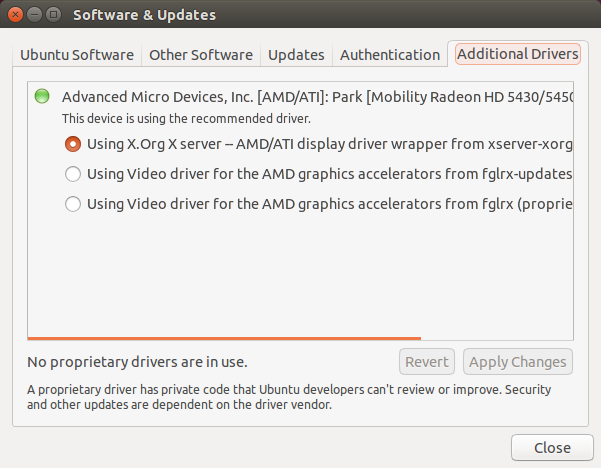
\includegraphics[scale=0.5]{pics/28.png}
\end{center}

\section{به‌روزرسانی لیست نرم‌افزارهای مخازن نرم‌افزاری}
در اوبونتو، برخلاف ویندوز، همهٔ نرم‌افزارهای موردنیاز را می‌توان از مخازن رسمی اوبونتو دانلود کرد. برای این‌که گنو/لینوکس‌تان از آخرین نسخهٔ نرم‌افزارها مطلع شود، لازم است لیست نرم‌افزارهای مخازن را به‌روز کنید. برای این کار، به اینترنت وصل شوید و برنامهٔ \lr{Terminal} را باز کنید و عبارت \lr{\texttt{sudo apt-get update}} را در آن تایپ کنید و کلید \lr{Enter} را بزنید. گذرواژه‌ٔ‌تان را وارد کنید (گذرواژه برای امنیت بیش‌تر، نشان داده نمی‌شود).

\begin{center}
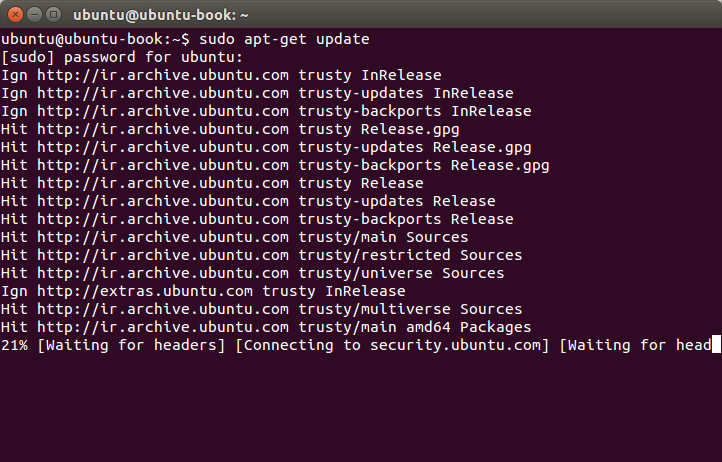
\includegraphics[scale=0.5]{pics/29.png}
\end{center}

\section[نصب کدک‌های چند رسانه‌ای، Flash Adobe و فونت‌های مناسب فارسی]{نصب کدک‌های چند رسانه‌ای، \lr{Adobe Flash} و فونت‌های مناسب فارسی}
اوبونتو بسیاری از کدک‌های صوتی و تصویری معروف مثل \lr{MP3}، فلش و \ldots  را به همراه ندارد. برای نصب آن‌ها، در مرکز نرم‌افزار (\lr{Software Center}) دنبال \lr{ubuntu-restricted-extras} بگردید و این بسته را نصب کنید.

\begin{center}
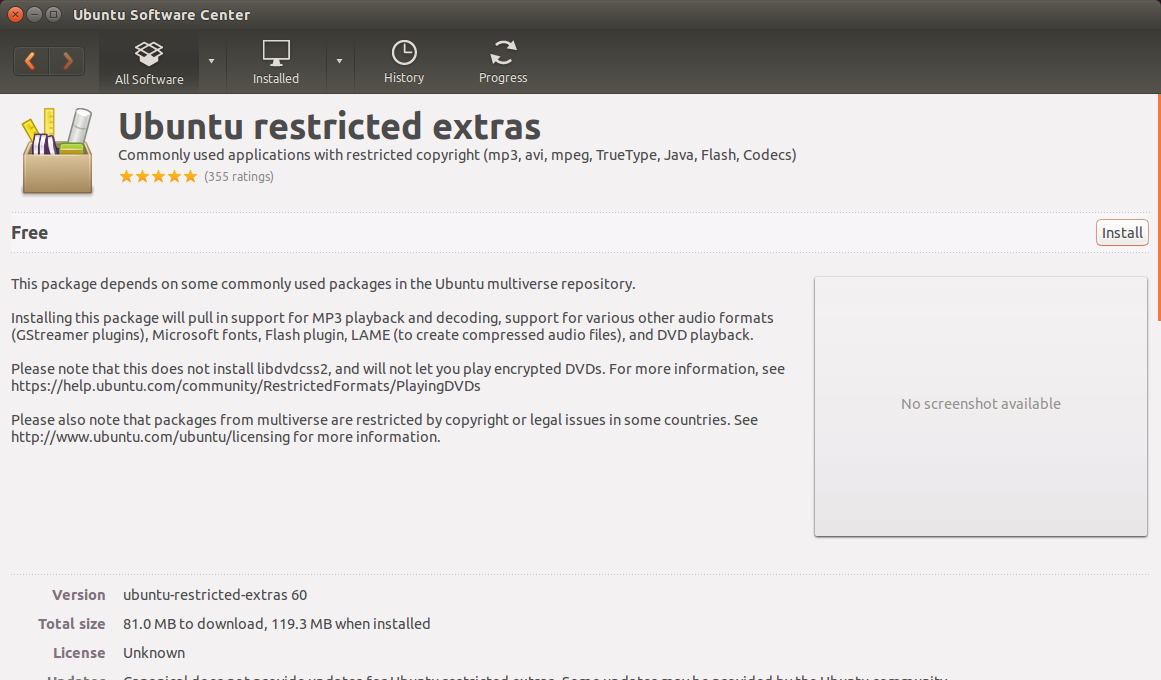
\includegraphics[scale=0.4]{pics/30.png}
\end{center}

\section{نصب برنامه‌های اضافی}
برنامه‌های همراه اوبونتو زیاد هستند، اما برای تمامی کارهای روزانه کفایت نمی‌کنند. صدها برنامهٔ آزاد و غیر آزاد وجود دارد که به راحتی یک کلیک از مرکز نرم‌افزار نصب می‌شوند. لیست زیر چند برنامهٔ پیشنهادی را معرفی می‌کند.
\begin{itemize}
\item \lr{Chromium}: مرورگر سریع کرومیوم
\item \lr{Gimp}: ابزاری قوی برای ویرایش و ساخت تصاویر پیکلسی، معادل \lr{Adobe Photoshop}
\item \lr{LibreCAD}: ابزار طراحی نقشه‌های ساختمانی، معادل \lr{AutoCAD}
\item \lr{GNU Octave}: ابزاری عالی برای رایانش عددی و تجسم داده، معادلی برای \lr{MATLAB}
\end{itemize}

\section{فعال‌کردن راست به چپ در لیبره‌آفیس}
برای این کار به این مسیر بروید:\\

\begin{center}
\lr{Langauges} \textsf{→} \lr{Language Settings} \textsf{→} \lr{Options} \textsf{→} \lr{Tools}\\
\end{center}

تیک گزینه \lr{Complex text layout (CTL)} را بزنید و سپس \lr{Persian} را از لیستی که فعال می‌شود، برگزینید.

\begin{center}
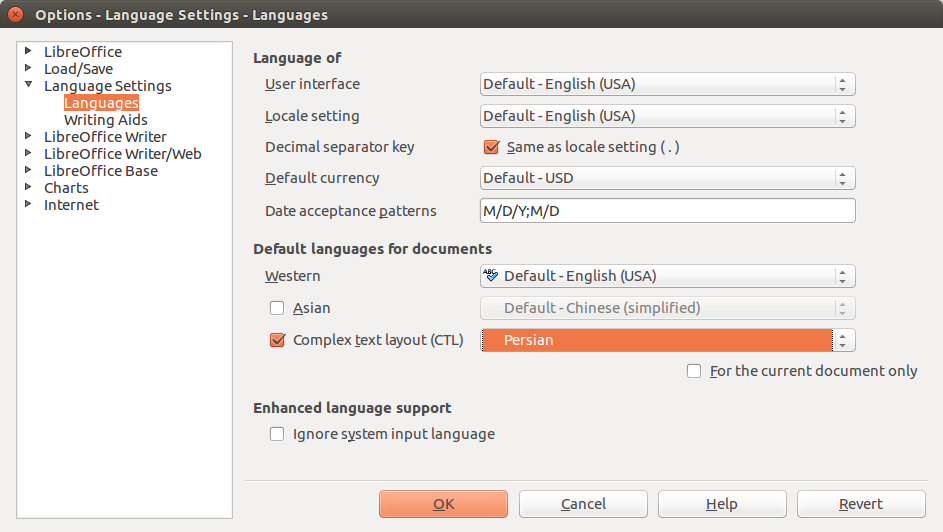
\includegraphics[scale=0.55]{pics/31.png}
\end{center}

\section{استفاده از میزکار متفاوت}
اوبونتو به همراه میزکار \lr{Unity} عرضه می‌شود، ولی آن را به شما تحمیل نمی‌کند. برای داشتن میزکار \lr{KDE}، بستهٔ \lr{kubuntu-desktop} و برای داشتن \lr{Gnome Shell}، بستهٔ \lr{gnome-shell} را نصب کنید.

\begin{center}
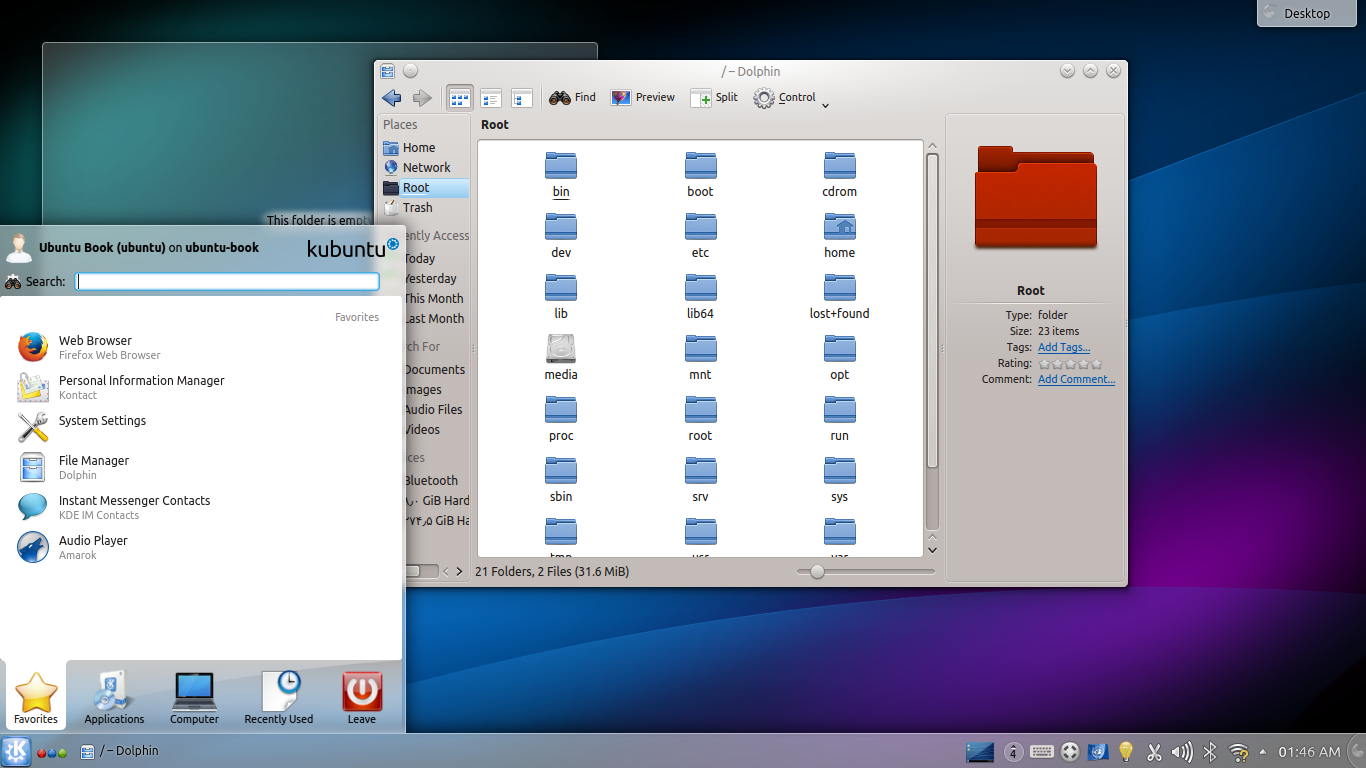
\includegraphics[scale=0.45]{pics/32.png}\\
نمایی از \lr{KDE}\\
\end{center}

\begin{center}
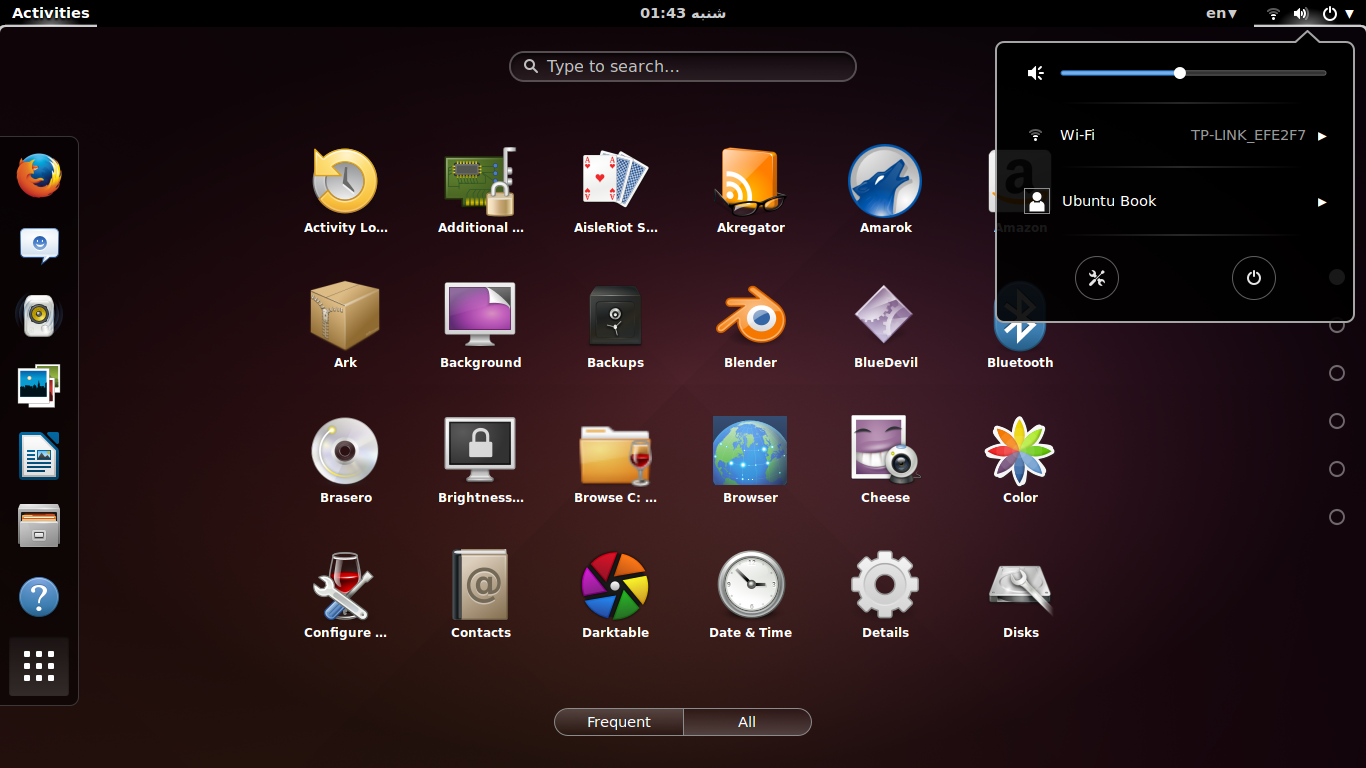
\includegraphics[scale=0.33]{pics/33.png}\\
نمایی از \lr{Gnome Shell}
\end{center}

\section{سفارشی‌سازی میزکار}
جدا از این‌که چه میزکاری استفاده می‌کنید، می‌شود آن را با مجموعهٔ آیکن، فونت و پوسته‌های مختلف شخصی‌سازی کرد. مجموعه‌ای از بهترین آیکن و پوسته‌ها را از \lr{gnome-look.org} و \lr{kde-look.org} بگیرید. راهنمای استفاده هم همان جا وجود دارد.
\begin{center}
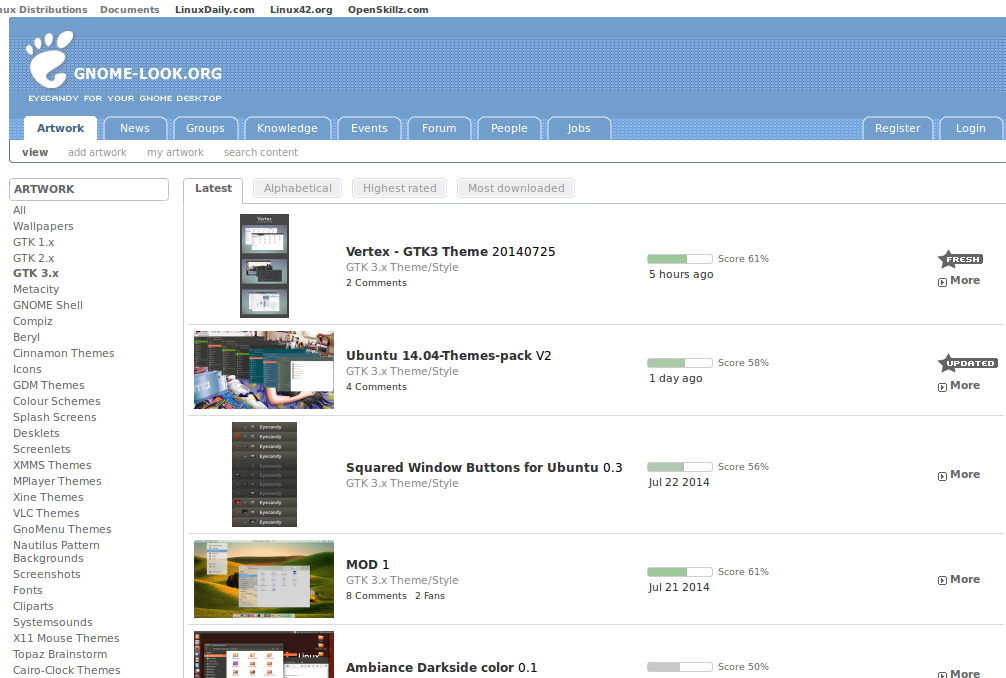
\includegraphics[scale=0.4]{pics/34.png}
\end{center}

\section{راه‌اندازی کلاینت ایمیل}
اوبونتو \lr{Thunderbird} را به همراه دارد که ابزاری برای مدیریت ایمیل‌هاست. بعد از اجرای تاندربرد، اسم، آدرس ایمیل و پسورد حساب ایمیل‌تان را به آن بدهید تا ایمیل‌هایتان را دریافت کند.

\section{همکاری در جامعهٔ کاربری اوبونتو}
اوبونتو با همکاری جامعهٔ کاربری‌اش زنده است و کتابی هم که می‌خوانید، با همکاری همین جامعهٔ کاربری ساخته شده است. تا جای ممکن، جامعهٔ کاربری را فراموش نکنید و به آن کمک کنید. \href{http://www.ubuntu.ir}{وب‌سایت فارسی اوبونتو} جای خوبی برای شروع است. تعداد بسیار زیادی سوال در انجمن بدون پاسخ مانده‌اند و ده‌ها مدخل در ویکی وجود دارد که نیازمند به‌روزرسانی است.

\section{معرفی اوبونتو به دوستان و آشنایان}
اوبونتو را به دوستان و همکاران‌تان معرفی کنید تا آن‌ها هم با این سیستم‌عامل فوق‌العاده و آزاد آشنا بشوند.
